\documentclass[12pt,a4paper,oneside]{article}
\usepackage[utf8]{inputenc}
\usepackage{t1enc} % hyphenate accented chars
\usepackage[hungarian]{babel}
\usepackage{../fedlap}
\usepackage{fancyhdr} % elofej, elolab
\usepackage{graphicx}
\usepackage{datetime} % specify date format
\setcounter{secnumdepth}{3} % enable subsubsection

% hasonlitson a doc verziora
\addtolength{\voffset}{-1cm}

% cim
\csapat{nand}{39}
\konzulens{Bozóki Szilárd}
\datum{\todaynum}

% csapattagok
\taga{Berki Endre}{HQNHER}{berkiendre@gmail.com}
\tagb{Fodor Bertalan Ferenc}{H4T1UX}{foberci@gmail.com}
\tagc{Kádár András}{JFENWR}{arycika@gmail.com}
\tagd{Thaler Benedek}{EDDO10}{thalerbenedek@gmail.com}

\setlength{\headheight}{1.3em}
\setlength{\headsep}{2em}

% elofej, elolab
\fancyhf{}

\fancyhead[OL] { \tiny \leftmark{} }
\fancyhead[OR] { \tmpcsapat }

\fancyfoot[OR] { \thepage }
\fancyfoot[OL] { \tmpdatum }

\pagestyle{fancy}

% custom date format, according to customer request
% you have to use the \todaynum command instead of today,
% becouse babel overrides it, and I couldn't find a way to override
% it again. I was tempted to call this format \todaybozoki
\newcommand{\todaynum}{\the\year. \twodigit\month. \twodigit\day}


\begin{document}

\anyag{2. Követelmény, projekt, funkcionalitás}
\fedlap
\tableofcontents

\addtocounter{section}{1}
\section{Követelmény, projekt, funkcionalitás}

\subsection{Követelmény definíció}

    \subsubsection{A program bemutatása, alapvető feladatai}
Az elkészített program egy nagymértékben logikai, kismértékben ügyességi játék, mely koncepcióját tekintve teljesen megfelel a Ragtime Games által fejlesztett Continuity játéknak\footnote{http://continuitygame.com/playcontinuity.html}. A játék során a játékos több pályán keresztül tesztelheti logikai és problémamegoldó készségét. Az előre kialakított pályákon az előrehaladás a keretek egymáshoz képest történő elmozdításával, a kereteken belül pedig egy figurával 2 dimenzióban végzett mozgással történik. Minden pálya egy $n*k$-s táblából áll, amin $n*k-1$ keret található. Az összeillő keretek között átjárás van, az üres hellyel szomszédos keretek átmozgathatóak az üres helyre. A játékos által irányított figurának a keretekben található kulcsokat kell összeszednie, hogy azzal a szintén a keretekben található ajtót kinyitva a pályát teljesítse.

    \subsubsection{Felhasználói felület}
A kész program grafikus felhasználói felülettel rendelkezik, melyen az indítással és működéssel kapcsolatos funkciók egy menüsoron keresztül érhetőek el, egér vagy billentyűzet segítségével. Maga a játék kizárólag billentyűzettel irányítható.

    \subsubsection{A program futtatásának követelményei}
A program futtatásához szükséges a futtató számítógépre telepített Java Runtime Environment (JRE), mely ingyenesen beszerezhető a gyártó honlapjáról\footnote{http://java.com/en/download/index.jsp} a legtöbb platformra. A program hardware követelménye megegyezik az Oracle által meghatározott minimum-konfigurációval\footnote{http://www.java.com/en/download/help/sysreq.xml}, mely szükségessé tesz egy kompatibilis operációs rendszert (Windows, Linux), rendszertől függően 64-128 MB memóriát és hozzávetőlegesen 100 MB szabad helyet.

    \subsubsection{A program telepítése}
A program futtatásához a kész terméket csupán a futtató számítógép merevlemezére kell másolni, további telepítés vagy beállítás nem szükséges, amennyiben a futtató számítógép megfelel a futtatás követelményeinek.

    \subsubsection{A program fordítása}
A program fordításához szükség van a \texttt{javac} programra, mellyel a \texttt{*.java} fájlok lefordíthatóak, és a futtatható \texttt{jar} fájl elkészíthető.
    
\subsection{Projekt terv}

    \subsubsection{Fejlesztőeszközök, erőforrások}
	A csapat választása az Eclipse\footnote{http://eclipse.org/} fejlesztői rendszerre esett, mert a java világ egyik legelterjedtebb, keresztplatformos IDE megoldása, melyet a csapat minden tagja használt már korábban. UML modellezéshez, diagramok készítéséhez a Visual Paradigm Community Edition\footnote{http://www.visual-paradigm.com/} kiadását fogjuk használni.
A dokumentáció \LaTeX -ben készül, mely segítségével nyomtatásban jól kinéző dokumentumok készíthetőek, valamint a forrásfájlok könnyen verziókezelhetőek. A végső fájlokat PDF formátumba fordítjuk, majd ezt kinyomtatva adjuk be. A verziókezelést és a felmerülő problémák megoldását a GitHub\footnote{https://github.com/} online és ingyenes felületen keresztül oldjuk meg.

    \subsubsection{A fejlesztőcsapat tagjai, feladatai}
	\begin{center}
	\begin{tabular} {| l | c | }
		\hline
		Név & Feladatok\\
		\hline
		Thaler Benedek & csapatvezetés, dokumentáció, diagramok készítése, kódírás \\ 
		\hline
		Berki Endre & dokumentáció, diagramok készítése, kódírás \\
		\hline
		Fodor Bertalan & dokumentáció, diagramok készítése, kódírás \\
		\hline
		Kádár András & dokumentáció, diagramok készítése, kódírás \\
		\hline
	\end{tabular}
	\end{center}
	A feladatkörök, beosztások változhatnak a személyes időráfordítástól függően. A feladatok elosztásakor a fő szempont, hogy a feladatokat egyenlően tudjuk elosztani, így minimalizálva az egy emberre eső terhelés mértékét.

    \subsubsection{Kommunikációs modell}

	A tárgy keretében, a projektbe válogatott csoport tagjai előzetesen ismerték egymást, az előzetes ismeretség megkönnyíti az együttműködést és a hatékony munkavégzést. A munkavégzést további kommunikációt segítő programok támogatják.
	A kommunikáció megszervezése elsődleges fontosságú, így minél előbb próbáltuk felépíteni a kommunikációs hálózatot. Két részre oszthatóak a felhasznált kapcsolatteremtési formák, egyik a szinkron, másik az aszinkron kommunikáció. Szinkron kommunikációban lehetséges a folyamatos kommunikálás, azonnali reagálással egymás ötleteire, kérdéseire. Látható, hogy minden csapattag egyidejű bevonása a kommunikációba költséges és gyakran felesleges, ezért az ilyen megbeszéléseket minimálisra szorítjuk. Emellett fontos az asszinkron kommunikációs eszközök használata, melyek segítségével a csapattagok egymás elérhetőségétől függetlenül üzenhetnek egymásnak. Ez a fajta kommunikáció megfelelő a státusz jelentések számára, valamint az előrehaladás követésére vagy a feladatok kiadására.
	A csapatmunka számára a legfontosabb rendszer a GitHub által biztosított tároló\footnote{https://github.com/nandinc/Continuity}. Ez egy összetett rendszer, amely többféle lehetőséget biztosít számunkra:
	\begin{description}
		\item[Git verziókezelés:]
			A dokumentum és kódkészítés folyamatában lehetőséget nyújt, hogy többen dolgozhassanak együttesen a projekten, mindig mindenki a legfrissebb verziót érje el, manuális változáskövetés nélkül. Ezen felül segít nyomonkövetni a csapattagok munkáját egy részletes napló segítségével. % commit szó nem szerepelhet
		\item[Hibajegy nyilvántartó:] % issue tracker nem szerepelhet
			A feladatok kiosztása hibajegyeken kereszül történik. Egy-egy hibajegy addig marad nyitva, ameddig a hozzárendelt csapattag a feladatot el nem készíti és azt egy másik le nem ellenőrzi. Ezután a hibajegy lezárásra kerül, de a rendszerben marad, így későbbi probléma esetén újra megnyitható. A hibajegyek használatával a csapatvezető könnyen rendelhet feladatokat a csapattagokhoz, valamint lehetőség van egy feladat önkéntes elvállalására is. A hibajegyben a feladója pontosan leírja a feladatot, feltünteti a felhasználható forrásokat és kiköti, hogy milyen körülmények teljesítése mellett zárható le a jegy.
		\item[Wiki:]
			Az értekezletek eredményeit, a csapattagok által készített segédleteket, fejlesztési irányelveket tároljuk itt.
	\end{description}
	Ezeken felül kommunikáció lehetséges a heti rendszerességgel tartott megbeszéléseken, Skype-konferencia formájában és egyéb személyes találkozókon. A teljes projekt döntéseit érintő kérdések megbeszélése valamint tervezési feladatok kidolgozása ezen szinkron kommunikációs formákban praktikusabb.

	\begin{figure}[h]
		\begin{center}
			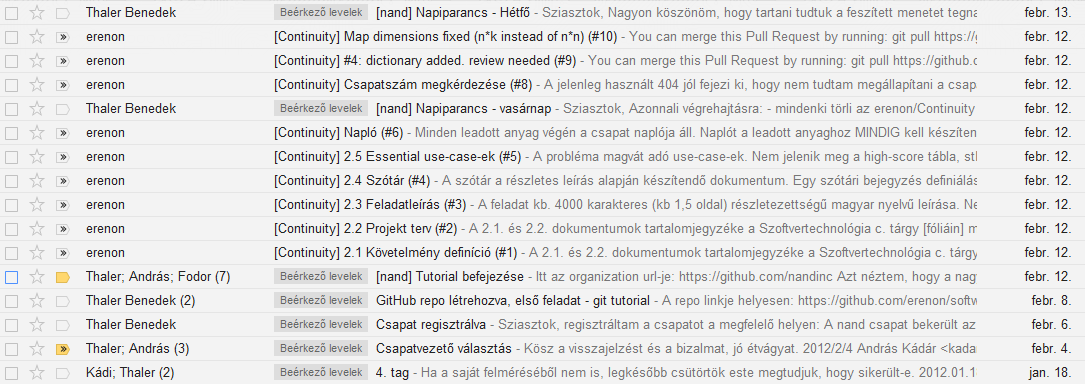
\includegraphics[scale=0.5]{resources/levlista.png}
			\caption{Levelezőlista}
		\end{center}
	\end{figure}
	
	\begin{figure}[h]
		\begin{center}
			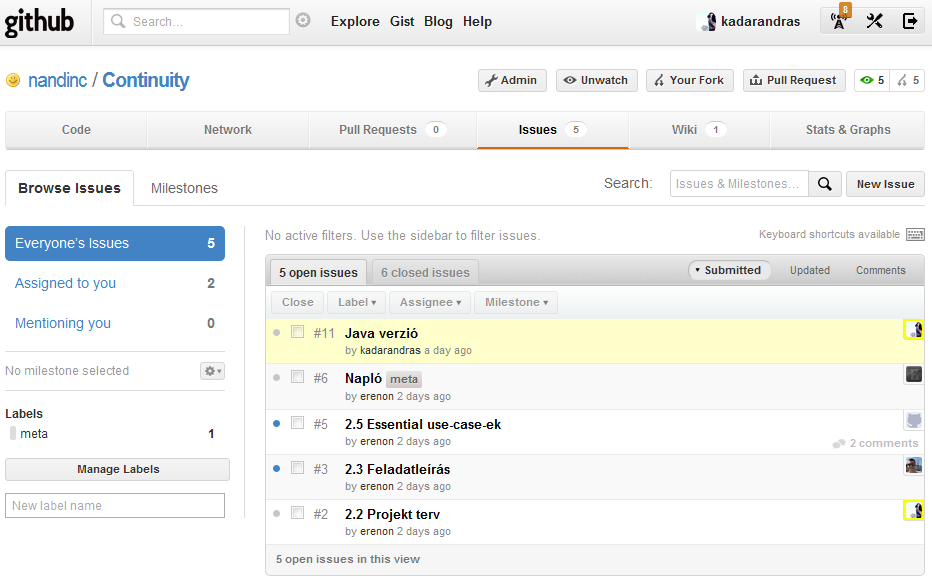
\includegraphics[scale=0.5]{resources/issues.png}
			\caption{A GitHub által biztosított hibajegykezelő}
		\end{center}
	\end{figure}

    \subsubsection{Fejlesztési mérföldkövek}

	\begin{description}
		\item[Szkeleton:] Az első fontosabb mérföldkő, a program vázának megalkotása, a program modelljének megtervezése, annak helyességének és részletességének ellenőrzése. A tervezési folyamat során fontos a gondos és odafigyelő döntéshozás, mert ezek a már elkészült program minőségét nagyban befolyásolják. Általánosságban igaz, hogy az itt elkövetett tervezői hibák később sokkal nagyobb erőfeszítéssel javíthatóak.
		
		\item[Prototípus:] A második mérföldkő a program működőképes változata, ami még a grafikát nem tartalmazza. A mérföldkő elérése a program egészének tesztelését teszi lehetővé. A fejlesztés ezen része lezárultnak tekinthető, ha az algoritmusok és adatszerkezetek, valamint az osztályhierarchia eléri végleges formáját, így egy a grafikus felülettől független programot alkot.
		
		\item[Grafikus felület:] A harmadik és egyben utolsó mérföldkövet a grafikus felület befejezése jelenti. A már kész, jól működő prototípust megfelelően felhasználva, azt meg nem bontva kell rá felépíteni a grafikus felületet. A felület fontos jellemzője az intuitív elrendezés, a felhasználó barát működés és könnyű használhatóság.
	\end{description}

    \subsubsection{Határidők}
	\begin{center}
	\begin{tabular}{| l | l | }
		\hline
		febr. 10. & 14 h -- csapatok regisztrációja\\
		\hline
		febr. 20. & Követelmény, projekt, funkcionalitás -- beadás\\
		\hline
		febr. 27. & Analízis modell kidolgozása 1. -- beadás\\
		\hline
		márc. 5. & Analízis modell kidolgozása 2. -- beadás\\
		\hline
		márc. 12. & Szkeleton tervezése -- beadás\\
		\hline
		márc. 19. & Szkeleton -- beadás\\
		\hline
		márc. 26. & Prototípus koncepciója -- beadás\\
		\hline
		ápr. 2. & Részletes tervek -- beadás\\
		\hline
		ápr. 16. & Prototípus -- beadás\\
		\hline
		ápr. 23. & Grafikus felület specifikációja -- beadás\\
		\hline
		máj. 7. & Grafikus változat -- beadás\\
		\hline
		máj. 11. & Összefoglalás -- beadás\\
		\hline
	\end{tabular}
	\end{center}

    \subsubsection{Átadás}
	A dokumentációt nyomtatott formában minden héten a konzulensnek le kell adni a konzultáció időpontjában. Ezen kívül a három mérföldkő alkalmával a programkódok is bemutatásra kerülnek az ezen célra kijelölt laboratórium gépeinél. A végső átadás a félév végeztével az aktualizált dokumentációval és forráskódokkal feltöltésre kerül a tárgy honlapjára\footnote{http://www.iit.bme.hu/hercules}.
%
%   \subsubsection{Kockázatelemzés}
%	\begin{description}
%	\item[Valószínűségek osztályozása:] \hfill \\
%		\begin{description}
%			\item[Alacsony] Közelítőleg 0-20\%-os eséllyel bekövetkező esemény
%			\item[Közepes] Közelítőleg 20-50\%-os eséllyel bekövetkező esemény
%			\item[Biztos] Közelítőleg 50-100\%-os eséllyel bekövetkező esemény
%		\end{description}
%	\item[Hatások osztályozása:] \hfill \\
%		\begin{description}
%			\item[Elhanyagolható] Az esemény bekövetkezése nem okoz különösebb problémát, az esetleges javítása nem igényel komoly munkálatokat.
%			\item[Enyhe] Az esemény bekövetkeztével okozott kár legfeljebb néhány munkaórával javítható, visszaállítható.
%			\item[Közepes] A csapat több tagjának összehangolt munkáját igénylő probléma, melynek megoldása komolyabb erőfeszítéseket igényel. Ezen változtatások már hatással lehetnek a heti ütemtervre, és a fejlesztőcsapat közös megbeszélését igényelhetik.
%			\item[Komoly] A projekt sikeres kimenetelét vagy a csapat integritását fenyegető esemény, mely alapvető változtatásokkal jár. Az ilyen jellegű probléma a csapat azonnali tanácskozását igényli.
%		\end{description}
%	\end{description}
%
%	Eseménytáblázat:
%	\begin{center}
%		\begin{tabular}{| l | l | l |}
%			\hline
%			\textbf{Esemény}			&	\textbf{Valószínűség}	&	\textbf{Hatás}\\
%			\hline
%			Specifikációváltozás			&	Biztos				&	Enyhe\\
%			\hline
%			Javítandó heti beadandó		&	Közepes			&	Enyhe\\
%			\hline
%			Sikertelen heti beadandó		&	Alacsony			&	Közepes\\
%			\hline
%			Csapattag kiválás			&	Alacsony			&	Komoly\\
%			\hline
%			Csapattag betegsége, távolléte	&	Alacsony			&	Közepes\\
%			\hline
%			Hardvermeghibásodás		&	Alacsony			&	Elhanyagolható\\
%			\hline
%			Szoftvermeghibásodás		&	Közepes			&	Enyhe\\
%			\hline
%			Határidorol lecsúszás		&	Alacsony			&	Közepes\\
%			\hline
%			Tanácskozásról hiányzás		&	Közepes			&	Közepes\\
%			\hline
%		\end{tabular}
%	\end{center}
%
   \subsubsection{Egyéb fontos megjegyzések}
	A fejlesztés lefordítása és bemutatása a HSZK laborjaiban történik, így a program forráskódjának kompatibilisnek kell lennie a Java Development Kit ennek megfelelő korábbi verziójával. A maximális kompatibilitás elérése érdekében a fejlesztés is pontosan ezeken a verziószámú platformokon történik majd, azaz 6-os Java JDK és 1.6.0 verziójú JRE kerül felhasználásra.

    \subsubsection{Szükséges dokumentációk}
	\begin{enumerate}
	\item Követelmény, projekt, funkcionalitás
	\item Analízis modell kidolgozása 1.
	\item Analízis modell kidolgozása 2.
	\item Szkeleton tervek
	\item Szkeleton
	\item Prototípus koncepciója
	\item Részletes tervek
	\item Prototípus
	\item Grafikus felület specifikációja
	\item Grafikus változat
	\end{enumerate}
 
\subsection{Feladatleírás}

	A feladat a Continuity\footnote{http://continuitygame.com/playcontinuity.html} nevű logikai játék elkészítése. A játékos feladata az általa irányított pálcikaembert (továbbiakban: Stickman) a kétdimenziós térben úgy navigálni, hogy az megszerezze a pályán elhelyezett összes kulcsot, majd átmenjen a piros ajtón, így jutva a következő szintre. A játék különlegessége abban rejlik, hogy a pályák egy puzzle-hoz hasonlóan kis elemekből épülnek fel, melyek bizonyos szabályok szerint a játékos által átrendezhetőek.
	
	A felhasználó a játék elindításakor a főképernyővel találja szemben magát, ahol lehetősége van új játékot kezdeményezni vagy -- amennyiben már korábban is játszott -- a már megkezdett játékot folytatni.
	
	A játék szintekből áll, minden szinthez egy pálya tartozik. A pályák keretekből (csempékből) épülnek fel, melyek táblázatszerűen helyezkednek el. Ez a táblázat -- pályától függően -- tetszőlegesen széles vagy magas lehet, azonban mindig van benne pontosan egy üres cella, ami arra szolgál, hogy a kereteket tologatni lehessen. Csak az üres cella melletti keretek tolhatóak át az üres helyre, amennyiben a Stickman nem lóg ki a mozgatandó keretből. Ugyanis előfordulhat, hogy emberünk egy másik keretbe átlóg, ekkor a keret elmozdítása a szétszakítását eredményezné -- erre azonban egy pusztán logikai játékban nincs lehetőség.
	
	%Egy keret mozgatásához két feltételnek szükséges teljesülnie. Ez akkor tehető meg, ha egyrészről van mellette üres hely (ide lehet a keretet tolni, kereteket felcserélni nem lehet), illetve másrészről ha Stickman nem éppen a keret határán tartózkodik, azaz csak félig a mozgatandó keretben.
	
	Keretek mozgatására akkor nyílik lehetőség, amikor a játékos pálya nézetben van; ez a nézet töltődik be közvetlenül a pálya elindítása után. Ebben a nézetben a játékos a teljes pályát átlátja, az összes keret megjelenik, és Stickman mozgása szüneteltetve van.
Stickman mozgatására a játékosnak a közeli nézetben van lehetősége. Ide a pálya nézetből lehet jutni a szóköz billentyű lenyomásával (ugyanígy lehet vissza is menni), és ekkor a képernyőn csak Stickman, valamint az aktuális -- nagyjából egy keret nagyságú -- környezete jelenik meg.
	
	Stickmant a játékos irányítja a billentyűzetének kurzorai segítségével. Amíg akadályba nem ütközik, mehet jobbra--balra, illetve ugorhat is, valamint ha elfogy alóla a talaj, akkor esni kezd. A mozgást a keretek közti átjárást szabályzó speciális szabályok nehezítik. Ha Stickman kerethatárra érkezik, akkor két eset lehetséges. Amennyiben a keretek az adott oldalon átjárhatóak, akkor szabadon folytathatja útját a másik keretbe. Ha az érintett keretek nem átjárhatóak vagy az érintett irányban már nincs több keret, akkor ha oldalsó határról van szó, visszapattan (a kerethatár akadályként viselkedik), ha alsóról, akkor a játékos kiesik. Két keret akkor átjárható, ha a csatlakozó szélükön a tereptárgyak elhelyezkedése megegyezik.
	
	A játékos kiesése azzal jár, hogy Stickman visszakerül az utolsó mentési ponthoz (ellenőrző pont). Ilyen mentési pont Stickmannek a pályához tartozó kiindulási helye, illetve a megszerzendő kulcsok helye. Amennyiben a játékot elmentjük, majd később folytatjuk, akkor is a mentési pont lesz a kiinduló pont.
	
	Játék közben mind a pálya nézetből és a közeli nézetből az escape gomb megnyomásával elő lehet hozni egy menüt, mellyel menteni lehet az aktuális állapotot, illetve vissza lehet térni a főképernyőre.
	% Restart levelt és Skip Levelt ugye nem akarjuk megvalósítani?
	
	A pályán különböző kulcsok vannak elhelyezve, melyeket a játékosnak az előrehaladáshoz meg kell szereznie. Ezt úgy teheti meg, ha Stickmant vezetve megérinti ezeket, azaz elhalad előttük. Ha megszerezte az összes kulcsot, akkor a pályán elhelyezett ajtót kell célba vennie. Az ajtó előtt való elhaladáskor -- amennyiben a játékosnál van az összes kulcs -- az ajtó automatikusan kinyílik és a pálya teljesítésre kerül. Amennyiben a játékos még nem szerezte meg az összes kulcsot, az ajtó kinyitása nem lehetséges.
	
	Pálya teljesítése esetén egy átvezető képernyő után rögtön sor kerül a következő pálya automatikus betöltésére. Amennyiben több pálya már nem létezik, úgy egy gratuláló megjegyzés után a főképernyőre tudunk visszajutni.

\subsection{Szótár}

\begin{description}

    \item[Játékos] A programot kezelő felhasználó
    \item[Számítógép] A programot futtató számítógép, mely megfelel a futtatás követelményeinek
    \item[Monitor] A \emph{számítógéphez} csatlakoztatott képernyő, melyen a futtatott program megjelenik
    \item[Pálya] A játékban való előrehaladás egysége. Minden pálya egy $n*k$ méretű táblázatból áll, melyben $n*k-1$ előre meghatározott \emph{keret} előre meghatározott helyen található. A fennmaradó helyen egy \emph{üres keret} található.
    \item[Keret] Egy \emph{pálya} több keretből áll. Minden keret \emph{elem}eket tartalmaz. A \emph{Keretek} egymáshoz képest \emph{átrendez}hetőek. Két érintkező keret között egyértelműen megállapítható, hogy \emph{átjárhatóak}-e. Amennyiben \emph{Stickman} a keret alsó szélét érinti úgy, hogy az \emph{aktuális keret} nem \emph{átjárható} az alatta található kerettel, vagy nincs alatta keret, akkor \emph{Stickman} \emph{kiesik}.
    \item[Átjárható] Két \emph{keret} átjárható, ha az érintkező oldalukon a \emph{platform}ok elhelyezkedése megegyezik.
    \item[Aktuális keret] Az a \emph{keret}, amiben a játékos lába tartózkodik.
    \item[Üres keret] Az üres keret biztosít lehetőséget arra, hogy vele helyet cserélve a \emph{keret}ek átrendezhetőek legyenek. Az üres keret nem rendelkezik vizuális reprezentációval, csupán távtartó funkciója van.
    \item[Elem] Egy \emph{keret} dinamikus vagy statikus alkotórészei; \emph{Stickman}, \emph{kulcs}, \emph{ajtó}, \emph{platform}.
    \item[Stickman] A játékban a \emph{játékos} által irányított emberformájú figura.
    \item[Kulcs] A \emph{játékos} által \emph{megszerez}hető \emph{elem}. A \emph{pályá}n található összes kulcs megszerzése után van lehetőség az \emph{ajtó} \emph{kinyit}ására.
    \item[Ajtó] Olyan \emph{elem}, melyet \emph{kinyit}va a pálya \emph{teljesít}ettnek tekinthető.
    \item[Platform] Olyan \emph{elem}, mely meghatározza a \emph{keret} bejárható és nem bejárható részeit. Egy 2 dimenziós objektum, melyen a \emph{játékos} irányítása szerint \emph{Stickman} mozoghat.
    \item[Megszerez] \emph{Stickman} egy megszerezhető \emph{elem}et megszerez, ha azt megérinti, azaz elhalad előtte. Egy \emph{elem} csak egyszer szerezhető meg, el nem veszíthető.
    \item[Kinyit] \emph{Stickman} az \emph{ajtó}t kinyithatja, ha \emph{megszerez}te a \emph{pályá}n található összes \emph{kulcs}ot. A kinyitás módja az ajtó megérintése. A kinyitás bekövetkeztekor a \emph{pálya} \emph{teljesít}ettnek tekinthető.
    \item[Teljesít (pályát)] A \emph{játékos} teljesíti a \emph{pályát}, ha \emph{kinyit}ja a pálya \emph{ajtaját}. Teljesítés után a \emph{következő pályá}ra léphet.
    \item[Kiesik] Ha \emph{Stickman} kiesik, akkor eltűnik, majd megjelenik az utolsó érintett \emph{ellenőrzőpont}nál
    \item[Ellenőrzőpont] Ellenőrzőpont a \emph{pálya} \emph{kezdőpont}ja, valamint minden \emph{kulcs} helye.
    \item[Kezdőpont] A \emph{pálya} egy pontja, ahol \emph{Stickman} először megjelenik a pálya betöltésekor.
    \item[Átrendez] Egy \emph{keret} átrendezhető, ha mellette \emph{üres keret} található és \emph{Stickman} csupán egy keretben jelenik meg. Ekkor a két \emph{keret} helye felcserélhető. Az átrendezést a \emph{játékos} vezérli.
    \item[Nézet] Meghatározza, hogy a \emph{játékos} az összes \emph{keret}et, (\emph{pálya nézet}) vagy csak a \emph{Stickman}t és közvetlen környezetét (\emph{közeli nézet}) lássa.
    \item[Pálya nézet] A \emph{játékos} az összes \emph{keret}et látja, és \emph{átrendez}ést kezdeményezhet.
    \item[Közeli nézet] A \emph{játékos} csak \emph{Stickman}t és -- nagyjából egy \emph{keret}nyi -- közvetlen környezetét látja, valamint vezérelheti a \emph{Stickman} mozgását.
    \item[Nézetváltás] A \emph{játékos} utasítására bármikor nézetváltás történhet, mely bekövetkeztekor a grafikus felület ráközelít az \emph{aktuális keret}re (\emph{Pálya nézet}ről \emph{Keret nézet}re váltás esetén) vagy eltávolodik az a \emph{Aktuális keret}ről az összes keret nézetére (\emph{Pálya nézet})
    \item[Nézetváltás] A \emph{játékos} utasítására bármikor nézetváltás történhet, mely bekövetkeztekor \emph{pálya nézet}ről \emph{közeli nézet}re váltás esetén a grafikus felület ráközelít \emph{Stickman}re, fordított esetben eltávolodik \emph{Stickman}től és a teljes pályát mutatja (\emph{pálya nézet}).
    \item[Következő pálya] Az aktuális \emph{pálya} után soron következő \emph{pálya} a \emph{pályalistá}ban.
    \item[Pályalista] A program által tartalmazott összes \emph{pálya} egy előre definiált sorrendben.

\end{description}


\clearpage
\subsection{Essential use-case-ek}
	\subsubsection{Essential use-case diagram}
	
		\begin{figure}[h!]
			\begin{center}
				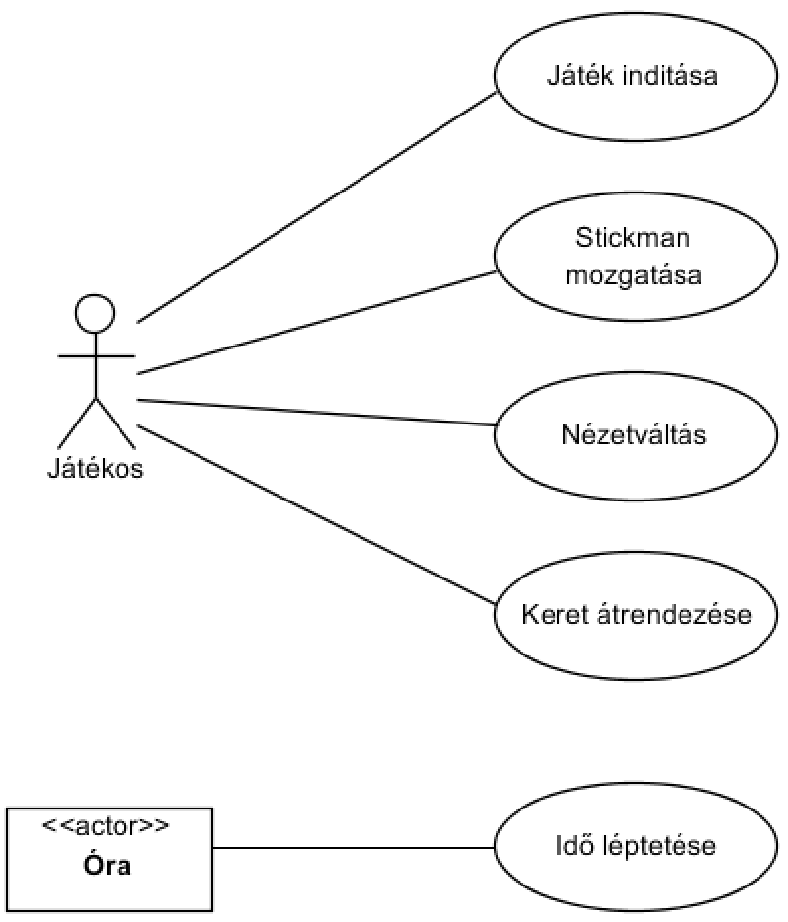
\includegraphics[scale=0.4]{resources/essential_use_cases.png}
				\caption{Alapvető use-case-ek}
			\end{center}
		\end{figure}
						
	\subsubsection{Essential use-case-ek leírása}
	
		\begin{description}
		
		\item[Játék indítása] \hfill \\
			A játékos folytatja a játékot, a legutóbbi, még teljesítetlen pálya töltődik be.
		\item[Stickman mozgatása]\hfill \\
			A játékos vezérli a figura (Stickman) mozgását. Stickman mozgatása a leütött billentyűnek megfelelően fog megtörténni.
		\item[Nézetváltás]\hfill \\
			A játékos a megfelelő billentyű lenyomásával nézetet vált (keret és pálya nézet).
		\item[Keret átrendezése]\hfill \\
			Keret nézetben a játékos a megfelelő billentyűkkel átrendezheti a pályát alkotó keretek helyzetét.
		\item[Idő léptetése]\hfill \\
			Egy számítógép által vezérelt actor végzi. Meghatározott időközönként jelzi az idő múlását, mely keret nézetben Stickman vertikális pozícióját befolyásolhatja.
		\end{description}

\end{document}
